%----------createClass----------------------------------------
\op
{createClass}
{creates a new class}
{createClass(Package selectedEObject, String nameValue)}
{The package providing the container for the newly created class.}
{
\begin{itemize}
 \item nameValue/newName: The name of the newly created class
 \item idValue/newID: The id of the newly created class
\end{itemize}
}
{There is no class whose name equals the parameter-value of 'newName' (see
\ref{subsec:checkOtherNames})}
{Only the name and the id will be set via input data. Visibility, isAbstract and
isFinal will be set with default values as defined with the diagram editor in
the image below.} \begin{figure}[H]
  \centering
  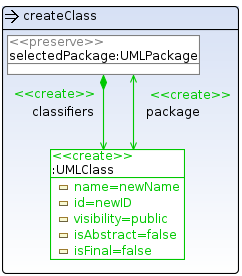
\includegraphics[width=0.4\textwidth]{pics/createClass.png}
  \caption{createClass}
  \label{createClass}
\end{figure}
%----------deleteClass----------------------------------------
\op
{deleteClass}
{Deletes a class}
{deleteClass(Class selectedEObject)}
{The class which should be deleted}
{-}
{-}
{For a better readability this is a simplified version of the
'deleteClass'-transformation and will only cover cases where the class
has no containments and no references to other elements. Such a complex
transformation rule exits but won't be listed here.}
\begin{figure}[H]
  \centering
  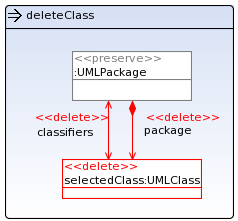
\includegraphics[width=0.4\textwidth]{pics/deleteClass_emptyAndUnreferenced.png}
  \caption{deleteClass}
  \label{deleteClass}
\end{figure}

%----------editClassName----------------------------------------
\op
{editClassName}
{edits the name of a class}
{editClassName(Class selectedEObject, String nameValue)}
{The class whose name should be renamed.}
{
\begin{itemize}
 \item nameValue/someName: The new name
\end{itemize}
}
{There is no class in the same package whose name equals the parameter-value of
'newName' (see
\ref{subsec:checkOtherNames})}
{The \textless\textless create\textgreater\textgreater  -symbol in the image
means that even if the attribute exists its value will be overwritten.
'someName' is the placeholder for the input name.}
\begin{figure}[H]
  \centering
  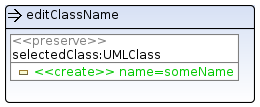
\includegraphics[width=0.45\textwidth]{pics/editClassName.png}
  \caption{editClassName}
  \label{editClassName}
\end{figure}
%----------editClassIsAbstract----------------------------------------
\op
{editClassIsAbstract}
{edits the isAbstract-value of a class}
{editClassIsAbstract(Class selectedEObject, boolean booleanValue)}
{The class whose isAbstract-value should be edited.}
{
\begin{itemize}
 \item booleanValue/bool: The new isAbstract-value
\end{itemize}
}
{-}
{The \textless\textless create\textgreater\textgreater  -symbol in the image
means that even if the attribute exists its value will be overwritten. 'bool'
is the placeholder for the input boolean value.}
\begin{figure}[H]
  \centering
  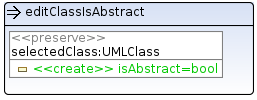
\includegraphics[width=0.45\textwidth]{pics/editClassIsAbstract.png}
  \caption{editClassIsAbstract}
  \label{editClassIsAbstract}
\end{figure}
%----------editClassIsFinal----------------------------------------
\op
{editClassIsFinal}
{edits the isFinal-value of a class}
{editClassIsFinal(Class selectedEObject, boolean booleanValue)}
{The class whose isFinal-value should be edited.}
{
\begin{itemize}
 \item booleanValue/bool: The new isFinal-value
\end{itemize}
}
{-}
{The \textless\textless create\textgreater\textgreater  -symbol in the image
means that even if the attribute exists its value will be overwritten. 'bool'
is the placeholder for the input boolean value.}
\begin{figure}[H]
  \centering
  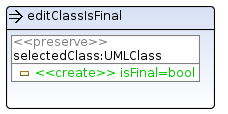
\includegraphics[width=0.40\textwidth]{pics/editClassIsFinal.png}
  \caption{editClassIsFinal}
  \label{editClassIsFinal}
\end{figure}
%----------editClassVisibility----------------------------------------
\op
{editClassVisibility}
{edits the visibility of a class}
{editClassVisibility(Class selectedEObject, Visibility visibilityValue)}
{The class whose visibility should be edited.}
{
\begin{itemize}
 \item visibilityValue/visibility: The new visiblility
\end{itemize}
}
{-}
{The \textless\textless create\textgreater\textgreater  -symbol in the image
means that even if the attribute exists its value will be overwritten.
'visibility' is the placeholder for the input visibility value.}
\begin{figure}[H]
  \centering
  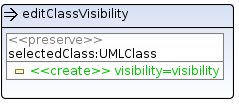
\includegraphics[width=0.40\textwidth]{pics/editClassVisibility.png}
  \caption{editClassVisibility}
  \label{editClassVisibility}
\end{figure}
%----------moveClass----------------------------------------
\op
{moveClass}
{moves a class from a package to another package}
{moveClass(Class selectedEObject, Package tgt)}
{The class which should be moved.}
{
\begin{itemize}
 \item tgt/tgt[moveClass]: the target package
\end{itemize}
}
{There is no class with the same name in the target context (see
\ref{subsec:checkOtherNames})}
{Only references will change.}
\begin{figure}[H]
  \centering
  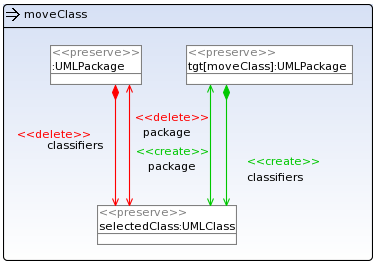
\includegraphics[width=0.65\textwidth]{pics/moveClass.png}
  \caption{moveClass}
  \label{moveClass}
\end{figure}